\section{Tema 6: Båndstruktur}
\label{tema6}


\begin{table}[!htb]
    \centering
    \caption{Samtale punkter tema 4}
    \begin{tabular}{|c|c|c|r|}
      \hline 
      1 & Fermi-Dirac fordelingen \& Båndstruktur i 1. Brilouisone & \autoref{sec:tema6_2} & \quad\quad \cellcolor{blue} \\
      \hline
      2 & Tilstandstetthet (DOS) & \autoref{sec:tema6_3} & \cellcolor{red} \\
      \hline
      3 & Elektron og hull i båndsrukturen & \autoref{sec:tema6_4} & \cellcolor{blue} \\
      \hline 
      4 & Båndstruktur i 3D & \autoref{sec:tema6_5} & \cellcolor{blue} \\
      \hline
      5 & Direkte og indirekte båndgap & \autoref{sec:tema6_6} & \cellcolor{blue} \\ 
      \hline
      6 & Forenklet bånddiagram & \autoref{sec:tema6_7} & \cellcolor{blue} \\
      \hline
    \end{tabular}
    \label{tab:samtalePunkt_tema1}
\end{table}


\subsection{Fermi-Dirac fordelingen \& Båndstruktur i 1. Brilouisone}
\label{sec:tema6_2}
Første Brillouinsone inneholder all informasjon vi trenger for elektroner i en krystall. En avbildning er illustrert i figur \ref{fig:infoBD}. Kurvene er ikke kontinuerlige, og sirkelene som er tegnet representerer elektroner, de ligger som ''perler på en snor''. 

\begin{figure}[!htb]
    \centering
    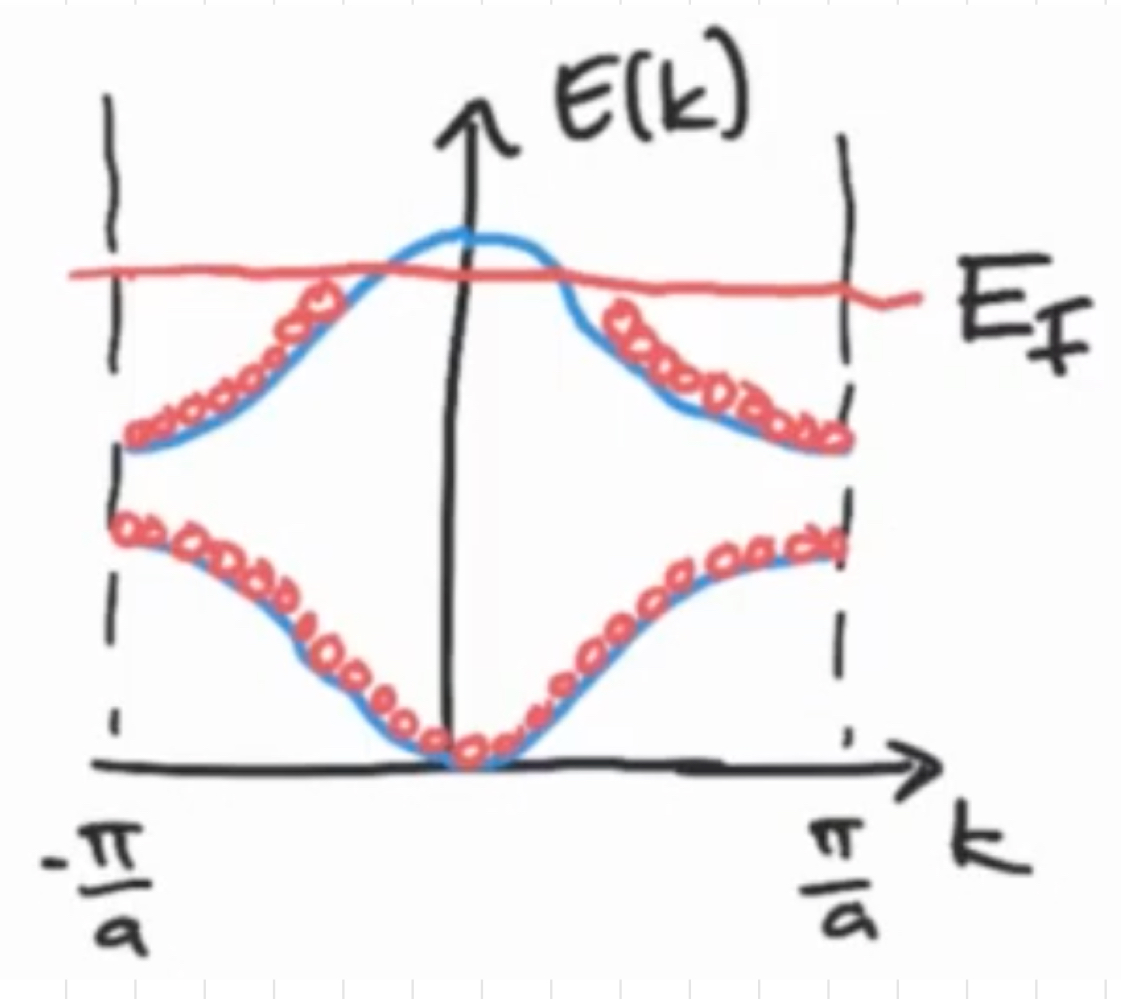
\includegraphics[scale=0.2]{Bilder/SamtaleTema6/infoBD.jpeg}
    \caption{1. Brillouin sone med elektroner tegnet på.}
    \label{fig:infoBD}
\end{figure}

NB! Det er $2N$ tilstander i hvert bånd, $N$ er antall energinivåer, og dette multipliseres med to siden det er mulig å ha spinn opp og spinn ned elektroner per energinivå.

En annen forklaring er at dette er elektroniske tilstander som alle har ulik $k$-verdi. Dette er Bloch bølger $\psi(x)=exp(ikx)u(x)$. Hvor $u$ har samme periodisitet som krystallen. 

Grunnen til vi velger å bruke elektroniske tilstander istedet for elektron er fordi man ved bruk av terminologien tar hensyn til den komplekse naturen til elektronets bevegelse i fast stoff. Elektroniske tilstander forklarer ikke bare den romlige posisjonen til elektron, men sier også noe om energi.

Eksempler på ulike elektroniske tilstander med ulik $k$-verdier kan være: 

\textbf{Valensbåndet}: Elektroniske tilstander nær bunnen av valensbåndet representerer tilstander der elektroner har lav energi ($k$ er liten, stor $\lambda$) og er bundet til kjernen.

\textbf{Ledningsbåndet}: Elektroniske tilstander nær toppen av ledningsbåndet har ulike $k$-verdier og representerer tilstander der elektronene har høy energi og er relativt fri til å bevege seg fritt gjennom krystallen.

Fra figur \ref{fig:infoBD} ser vi $E_F$, dette er fermienergien. Fermienergien forteller oss at ved $\SI{0}{\kelvin}$ er alle tilstander over $E_F$ tomme, mens alle tilstander under $E_F$ er fyllt opp, dette er fordi ved $\SI{0}{\kelvin}$ er det ingen termisk energi tilstedet. Vi kan ved bruk av dette produsere en sannsynlighetsfordeling for hvor vi kan finne elektroner.

\textbf{Fermi-Dirac-fordelingen} er en sannsynlighetsfordeling som beskriver uskarpheten ved fylling av tilstander.

\begin{empheq}[box=\tcbhighmath]{align}
    \label{eq:fermi-dirac}
    f(E) = \frac{1}{1+e^{\frac{(E-E_F)}{k_{b}T}}}
\end{empheq}

Funksjonen består av $k_b$ som er boltzmanns konstant, $T$ er temperaturen til krystallen. $E_F$ er fermienergien og $E$ er energien vi vil se om et elektron kan inneha. Denne funksjonen er da også en funksjon av temperaturen, da den produserer en helt ny sannsynlighetsfordeling. Vi ser at for $T=\SI{0}{\kelvin}$ får vi

\begin{equation}
\label{eq:potInfinite}
f(E) = \left\{
        \begin{array}{ll}
            0 & \quad E > E_F \\
            1 & \quad E < E_F
        \end{array}
    \right.
\end{equation}

Vi ser at $T=\SI{0}{\kelvin}$ er fordelingen en unit step function. \autoref{fig:fermiDirac} viser Fermi-Dirac fordelingen ved forskjellige temperaturer $T$.

\begin{figure}[!htb]
    \centering
    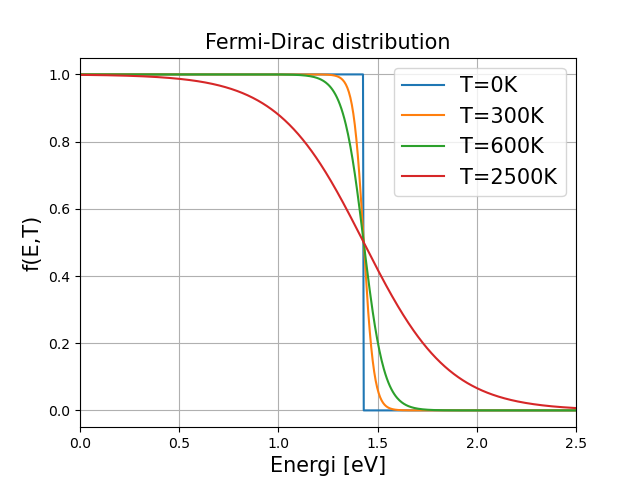
\includegraphics[scale=0.8]{Bilder/SamtaleTema6/fermiDirac.png}
    \caption{Fermi-Dirac fordelingen ved forskjellige temperaturer.}
    \label{fig:fermiDirac}
\end{figure}

La oss ta et eksempel der vi har to materialer, det ene har $E_F$ mot det øvre delen av valens båndet, som vi kaller det mat. \textcircled{1}, det andre har $E_F$ midt mellom valens bånd og ledningsbånd, vi kaller dette for mat. \textcircled{2}.

\textcircled{1} og \textcircled{2} kommer til å oppføre seg veldig forskjellig. \autoref{fig:sammenligning} viser de to materialene. ser vi på $x$-aksen har man ulike $k$, dette har noe med bevegelsesmengden å gjøre (husk at dette er krystall bevegelselsesmengden). Elektronene på positiv side har bevegelsesmengde i positiv $k$-retning, og dette handler om gruppehastigheten til Blochbølgene.

\begin{figure}[!htb]
    \centering
    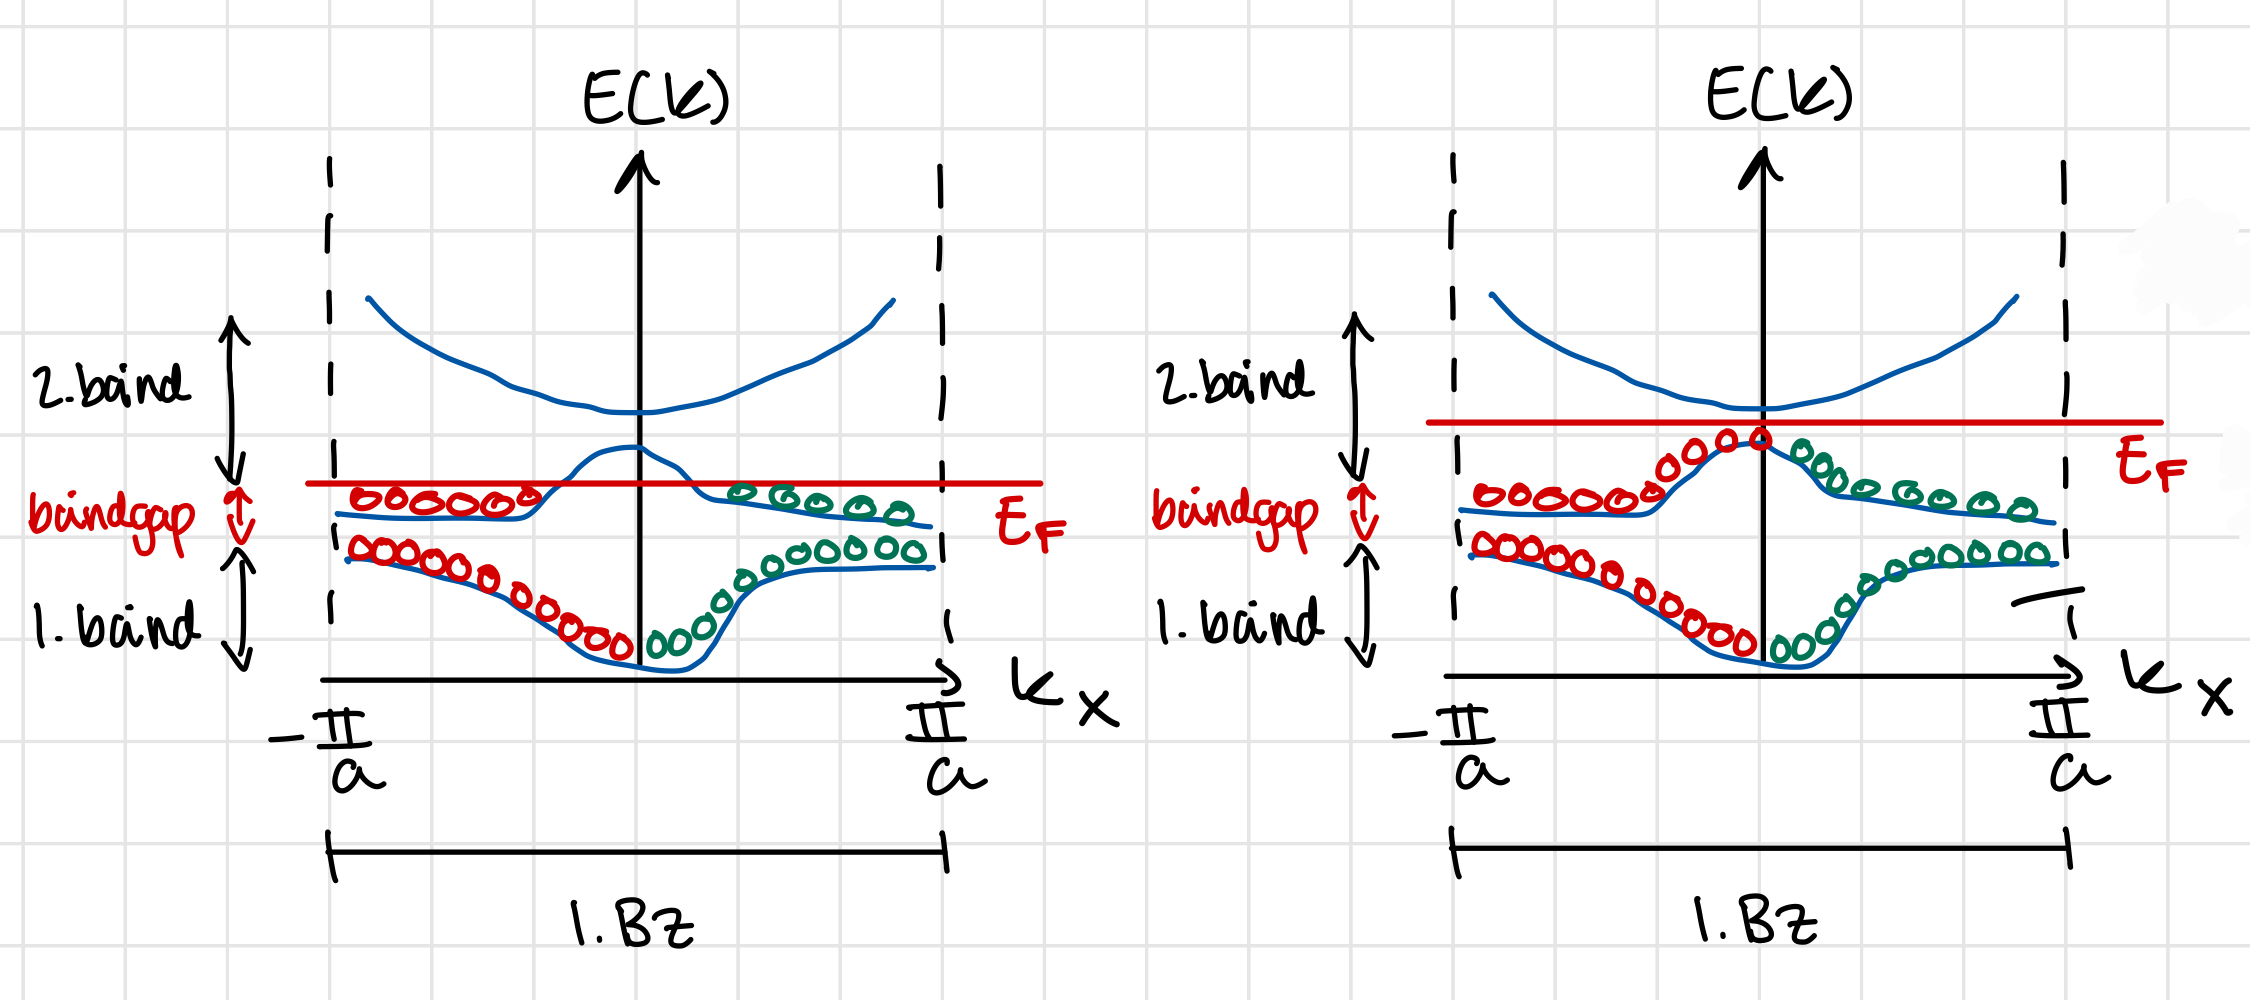
\includegraphics[scale=0.2]{Bilder/SamtaleTema6/sammenligning.jpeg}
    \caption{Venstre har vi mat. \textcircled{1}, og til høyre har vi mat. \textcircled{2}.}
    \label{fig:sammenligning}
\end{figure}

Et eksempel på mat. \textcircled{2} er silisium, de elektronene med bevegelsesmengde i positiv $k$-retning representerer bølgepakker/elektroner som beveger seg inni silisiumkrystallen. Desto større bevegelsesmengde, jo lengre unne origo er elektronet (større $k$), tilsvarende for elektroner i negativ $k$-retning, men da med negative fortegn.

\newpage
For mat. \textcircled{1} ser vi at båndstrukturen er usymetrisk, dette medfører til at netto bevegelselmengde ikke er null

\begin{equation*}
    \sum_i^N p_i \neq 0, 
\end{equation*}

Dersom båndene var like fulle på begge sider av $k=0$, slik som i mat. \textcircled{2}, får vi 

\begin{equation*}
    \sum_i^N p_i = 0, 
\end{equation*}

Dette gir en netto null ladningstransport. Vi kan med det si at mat. \textcircled{1} leder strøm bra, og vi kan si det er et metallisk materiale. Mat. \textcircled{2} leder ikke strøm bra, og vi kan si det oppfører seg som en isolator i utgangspunktet. Om båndgapet ikke er for stort kan vi si det er halvleder, dette er fordi det ikke krever veldig mye for et elektron å ''hoppe'' opp i ledningsbåndet.

\subsection{Tilstandstetthet (DOS)}
\label{sec:tema6_3}
Fylling av båndstrukturen er avgjørende for et materrial sine elektriske egenskaper

Metaller har halvfulle bånd, og leder derfor strøm godt. Isolatorer har fulle valens bånd, og tomme ledningsbånd og leder derfor ikke strøm. Vi er interessert i halvledere (som silisium). I utgangspunktet så har de fulle valensbånd, og tomme ledningsbånd, men det kreves lite energi for å overføre noen $e^-$fra øverste fylte båndt (VBM) til CBM. Det er slik silisium oppnår ledningsevne.

Så elektroner i ledgningsbåndet er det som kan gi ladningstransport. Det kan også være ''hullene'' som er i valensbåndet.

Vi er interessert i tallet på $e^-$ som er i CB, og antall hull i VB. For å finne disse, må vi koombinere informasjon fra båndstrukturen og Fermi-Dirac fordelingen. Ved å telle opp produktet av tilgjengelig plass og sannsynligheten for at denne er fylt, dette gir oss følgende integral.

\begin{equation}
    n(E) = \int_{0}^{\infty} g(E) \cdot f(E) dE
\end{equation}

$n(E)$ forteller os tettheten av $e^-$ i CB. Vi integrerer over alle mulige energinivå, $g(E)$ er density of states, denne funksjonen gir oss tettheten av tilstander for en viss energi. og $f(E)$ er sannsynligheten for å finne et elektron gitt en hvis energi.

I et båndgap er $g(E)=0$, fordi det ikke finnes noen mulige tilstander i båndgapet. Verdien på $g(E)$ avhenger av hvor tett elektronene ligger langs $k$-aksen. Vi antar at formen på båndene er parabler, dette er ikke en spesielt god antakelse, men den er god nok i de ''spennende'' områdene. 

Hvor tett tilstandene ligger, avhenger av krystallen. Man kan se dette ved hjelp av to metoder, begge gir samme $g(E)$ til slutt.

La oss anta at vi har en krystall som er rektangulær, med sider $L_x,L_y$ og $L_z$ og volum $V=L_xL_yL_z$. Med periodiske grensebetingelser får vi 

\begin{equation*}
    \psi(x+L_x,y,z) = \psi(x,y+L_y,z) = \psi(x,y,z+L_z) = \psi(x,y,z)
\end{equation*}

Setter vi dette inn i blochs toerem får vi

\begin{equation*}
    \exp{ik_xL_x} = \exp{ik_yL_y} = \exp{ik_zL_z} = 1    
\end{equation*}

Vi vet da at produktet av $k_j$ og $L_j$ må være heltall to pi, altså

\begin{equation*}
    k_x=\frac{2\pi}{L_x}n_x, \quad k_y = \frac{2\pi}{L_y}n_y, \quad
    k_z = \frac{2\pi}{L_z}n_z
\end{equation*}

Der $n_x,n_y,n_z=0,\pm 1, ..., N$. Vi ser at disse $k_j$ene er komponenter i bølgevektoren $\Vec{k}$, og vi kan med det si at produktet av alle tre gir oss the minste volumnet i $k$-rommet.

\begin{equation*}
    \frac{(2\pi)^3}{L_xL_yL_z} = \frac{(2\pi)^3}{V}
\end{equation*}

Vi vet at det er akkurat ett gitter punkt tilstede i dette volumet, fra det kan man trekke konklusjonen at tettheten av tillatte $\Vec{k}$ er uniform og lik $\frac{V}{(2\pi)^3}$ i $k$-rommet. Dette gir oss uttrykket 

\begin{equation}
    \label{eq:kTett}
    g(\Vec{k}) = 2 \frac{V}{(2\pi)^3}
\end{equation}

der faktoren to kommer fra spinn opp spinn ned karakteristikken til elektroner. $g(\Vec{k})$ er funksjonen som forteller oss om tettheten i $k$-rommet, denne er koblet opp mot funksjonen vi ønsker å finne $g(E)$. Forholdet mellom de to kan ser ut som

\begin{equation}
    \label{eq:forhold}
    g(E)dE = g(\Vec{k})d\Vec{k}
\end{equation}

her er $dE$ og $d\Vec{k}$ små intervaller av hhv. energi og enhetsvolum i $k$-rommet. For å finne $g(E)$ må vi vite forholdet mellom energien og $k$-rommet. Vi kan ta i bruk uttrykket vi har for energi, siden vi er interessert i området som er omtrent likt en parabel. 

\begin{equation}
\label{eq:energi_utledning}
    \begin{split}
        E(\Vec{k}) &= \frac{\hbar^2 k^2}{2m^*} \\
        dE &= \frac{\hbar^2}{2m^*}(2k)dk
    \end{split}
\end{equation}

Hvis vi tar i bruk sfæriske koordinater, kan vi skrive om $d\Vec{k}$ til

\begin{equation}
    \begin{split}
        d\Vec{k} &= d \bigg( \frac{4\pi}{3}k^3\bigg) \\
        d\Vec{k} &= 4\pi k^2 dk
    \end{split}
\end{equation}

Setter vi dette resultatet inn i ligning \ref{eq:energi_utledning}, får vi 
\begin{equation}
    \label{eq:dE}
    dE = \frac{\hbar^2}{2m^*} \bigg( \frac{1}{2\pi k}\bigg) d\Vec{k}
\end{equation}

Tar vi i bruk uttrykket for energi kan vi skrive det om mhp. $k$ og sette inn i ligning \ref{eq:dE}.

\begin{equation}
\label{eq:dEFin}
    dE = \frac{1}{2\pi}\bigg(
    \frac{\hbar^2}{2m^*}\bigg)^{\frac{3}{2}}
    \frac{1}{\sqrt{E}} d\Vec{k}
\end{equation}

Setter vi inn ligning \ref{eq:forhold} får vi 

\begin{equation}
    \label{eq:5.39.2}
    g(E) = 2\pi \bigg(
    \frac{2m^*}{\hbar^2} \bigg)^{\frac{3}{2}} \sqrt{E}g(\Vec{k})
\end{equation}

og ved å ta i bruk ligning \ref{eq:kTett} ender vi med

\begin{equation}
    \label{eq:tetthetFunc}
    g(E) = \frac{V}{2\pi^2}\bigg(\frac{2m^*}{\hbar^2}\bigg)^{\frac{3}{2}} \sqrt{E}
\end{equation}

Vi definerer ofte $g(E)=0$ ved ferminivået. Ferminivået er det interessante området der materialer går mellom ikke-ledende og ledende.

\begin{figure}[!htb]
    \centering
    \subfloat[\centering Tilstandstetthen \ref{eq:even}]{{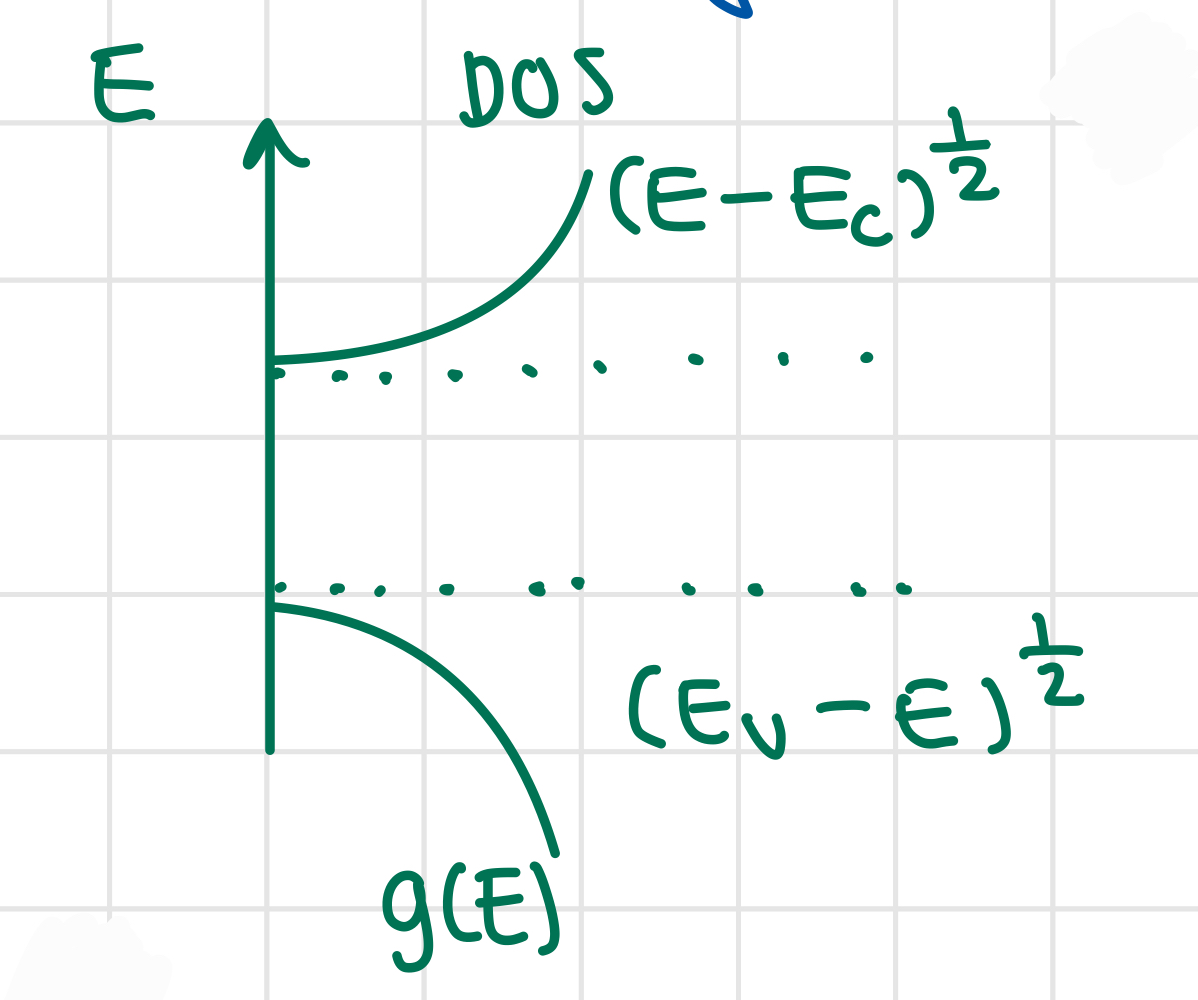
\includegraphics[width=7cm]{Bilder/SamtaleTema6/dosgraf.jpeg} }}%
    \qquad
    \subfloat[\centering $g(E)\cdot f(E)$ \ref{eq:odd}]{{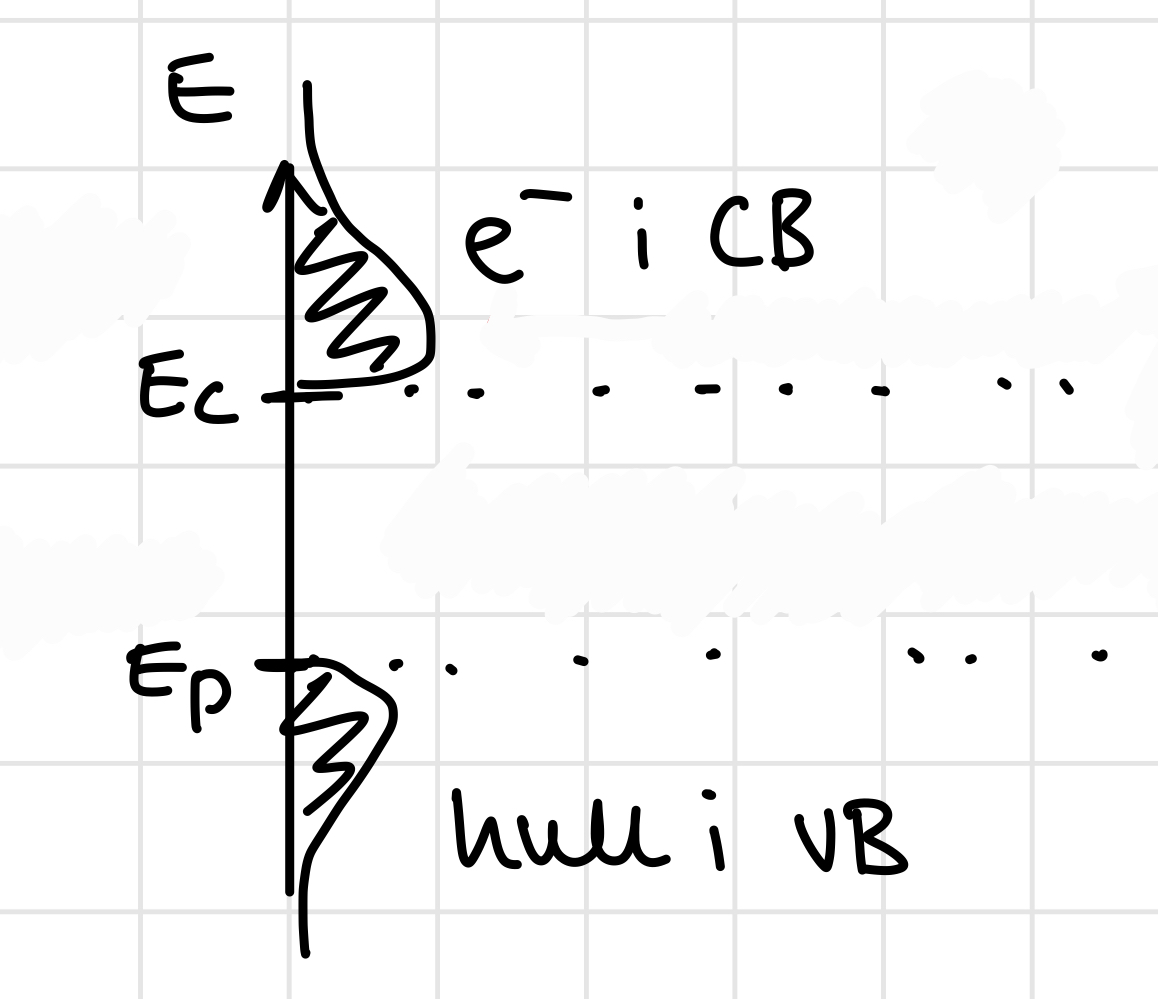
\includegraphics[width=7cm]{Bilder/SamtaleTema6/g(E)f(E).jpeg} }}%
    \caption{Tilstandstettheten $g(E)$ til venstre, og produktet av tilstandstetthen og Fermi-Dirac til høyre}%
    \label{fig:dobbelgreie}%
\end{figure}

\begin{figure}[!htb]
    \centering
    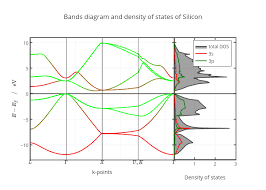
\includegraphics[scale=1.5]{Bilder/SamtaleTema6/DOS.png}
    \caption{Tilstandstettheten(DOS) for silisium på venstre side, plotet sammen med bånd diagrammet.}
    \label{fig:DOS_plot}
\end{figure}


Vi ser fra figur \ref{fig:dobbelgreie} at produktet av fermi-dirac fordelingen og tilstandstettheten avtar relativt raskt, dette produktet kallses ladningsbærertettheten og forteller oss antall ladningsbærere per volum. Dette inkluderer hull i valensbåndet da dette også kan ses på som ladningsbærere.

\newpage
\subsection{Elektron og hull i båndsrukturen}
\label{sec:tema6_4}
Elektroner befinner seg i ulike energibånd i et faststoff, det høyeste energibåndet som er fylt av elektroner ved lav temperatur kalles valensbåndet. Elektroner i valensbåndet har bundne tilstander. og de bidrar ikke uten videre til elektrisk ledning. Ved påvirkning fra ytre faktorer, som f.eks spenning, kan elektroner eksiteres til høyere energier, eller opp til ledningsbåndet, her kan de bevege seg friere og bidra til elektrisk ledning.

Et hull er et fravær av et elektron i valensbåndet, det oppfører seg som en positivt ladet partikkel. Hull kan bevege seg gjennom krystallen, og de kan betraktes som positive ladningsbærere. Når et elektron hopper fra valensbåndet til ledningsbåndet, etterlater det seg hull i valensbåndet som kan bevege seg gjennom krystallen og bidra til elektrisk ledning.

\subsection{Båndstruktur i 3D}
\label{sec:tema6_5}
Tidligere i dokumentet har vi produsert situasjoner ved hjelp av to dimensjoner, en for $k$-rommet, og en for energien $E(k)$, men nå vil vi inn i 3D for å tegne ekte faststoff. Vi kan prøve å lage en 3D tegning

\begin{figure}[!htb]
    \centering
    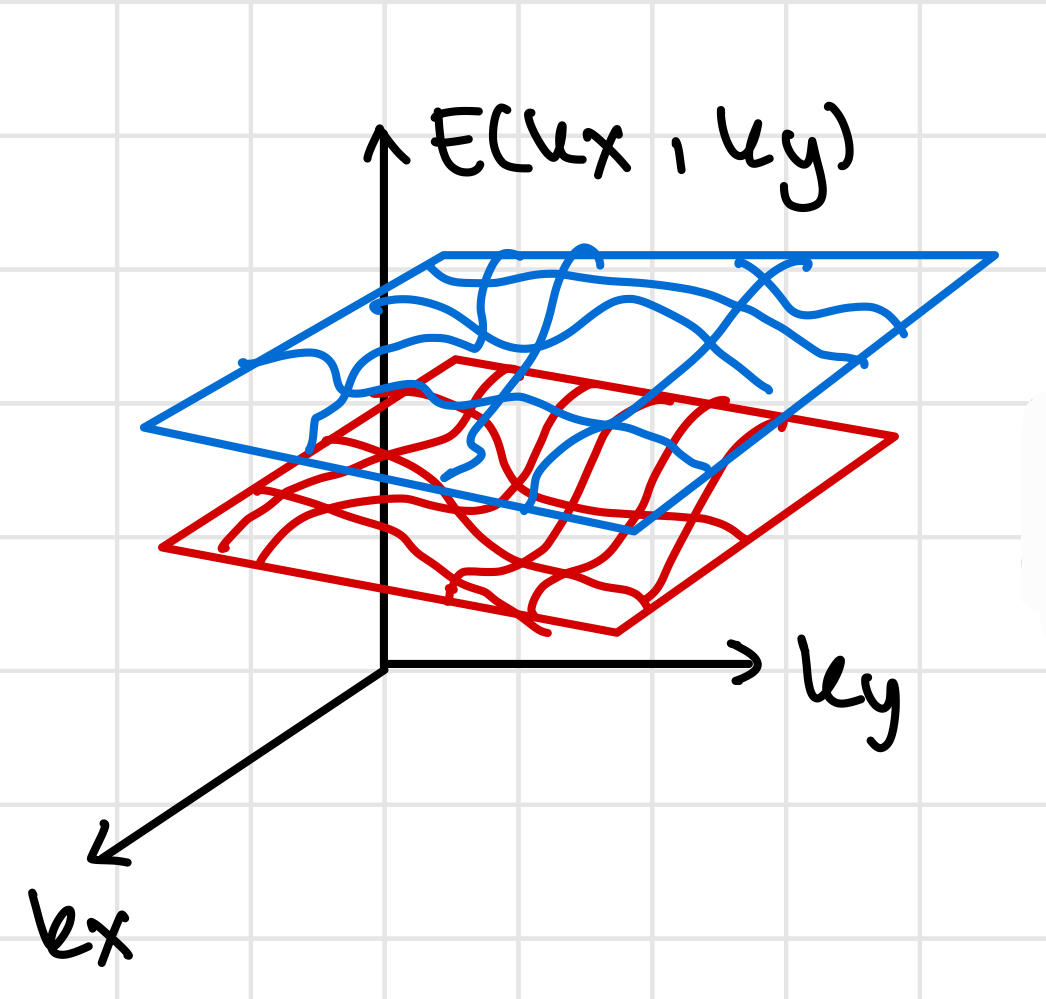
\includegraphics[scale=0.2]{Bilder/SamtaleTema6/2d-bandstruct.jpeg}
    \caption{Forsøk på 2D tegning...}
    \label{fig:2d_tegning}
\end{figure}

\autoref{fig:2d_tegning} så ikke så ille ut, men vi må jo lage 3 av disse, en til for $(k_x,k_z)$ og en for $(k_y,k_z)$. Vi prøver derfor noe litt annet, la oss heller si at vi går i en retning i $k$-rommet istedet, og grafer dette, så i en annen retning og tegner mens vi går rundt. Dette produserer figur \ref{fig:si_band}



\begin{figure}[!htb]
    \centering
    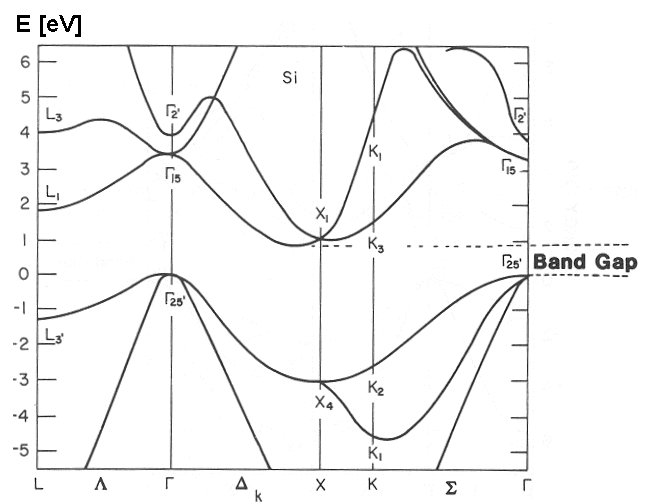
\includegraphics[scale=0.55]{Bilder/SamtaleTema6/si_banddiagram.png}
    \caption{Silisium sitt bånddiagram.}
    \label{fig:si_band}
\end{figure}


\begin{figure}[!htb]
    \centering
    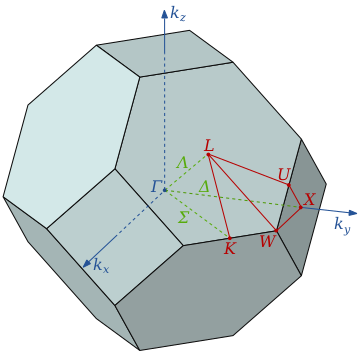
\includegraphics[scale=0.55]{Bilder/SamtaleTema6/brillouinZone.png}
    \caption{Første brillouin sone visualisert i 3D, Firkantene er flatsidene mellom to enhetsceller, sekskantene representerer bragg plan.}
    \label{fig:BZ}
\end{figure}

$\Gamma$ er sentrum, alle de greske bokstavene som dukker opp i figur \ref{fig:BZ} dukker også opp i figur \ref{fig:si_band}, dette hører med retningen de går rundt i rommet. 

\subsection{Direkte og indirekte båndgap}
\label{sec:tema6_6}
Et båndgap er avstanden mellom VBM og CBM (eller to vilkårlige bånd, men vi bryr oss om VBM og CBM).

Om $k$-vektoren til VBM er lik den i CBM, kalles det et \textit{direkte båndgap}, men om de ikke er like kalles det et \textit{indirekte båndgap}.

For direkte båndgap må krystallmomentet k (husk $p_{krystall}=\hbar k$) være likt VBM og CBM, dette gjør at elektroner i VBM kan ''hoppe'' direkte til CBM, de trenger ikke bevege seg til siden i k-rommet, altså de trenger ikke tilførsel av bevegelsesmengde. Dette kan gjøres ved tilførsel av energi i form av et foton.

For indirekte båndgap er ikke $k$-vektorene like, dette gjør at krystallmomentet i VBM og CBM er ulikt. Siden momentet er uliktt må noe av momentet til elektronet overføres til gitteret før det tar plass i CBM. For å eksitere et elektron i et indirekte båndgap, kan vi introdusere energi til systemet som kan omgjøres til bevegelsesmengde, for eksempel akkustiske bølger, dette vil produsere gitter vibrasjoner, noe som gir oss et høyere krystall moment. Elektroner inneholder ikke en stor bevegelsesmengde, så det må en kombinasjon av disse til for å eksitere ved et indirekte båndgap. 

Eksitering i et direkte båndgap gjøres ofte med fotoner, men ofte har fotoner litt mer energi enn det som egentlig trengs for eksitasjonen fra VBM til CBM, derfor frigjøres den ekstra energien ofte som fotoner. Dette gjør at halvledere med direkte båndgap egner seg godt i bruk i optiske komponenter som LED, lasere og solceller. 

\subsection{Forenklet bånddiagram}
\label{sec:tema6_7}
Forenklede bånddiagram er nyttige, det er enklere å visualisere ved å se på en diode av typen p-n, som illustrert i figur \ref{fig:p-n}

\begin{figure}[!htb]
    \centering
    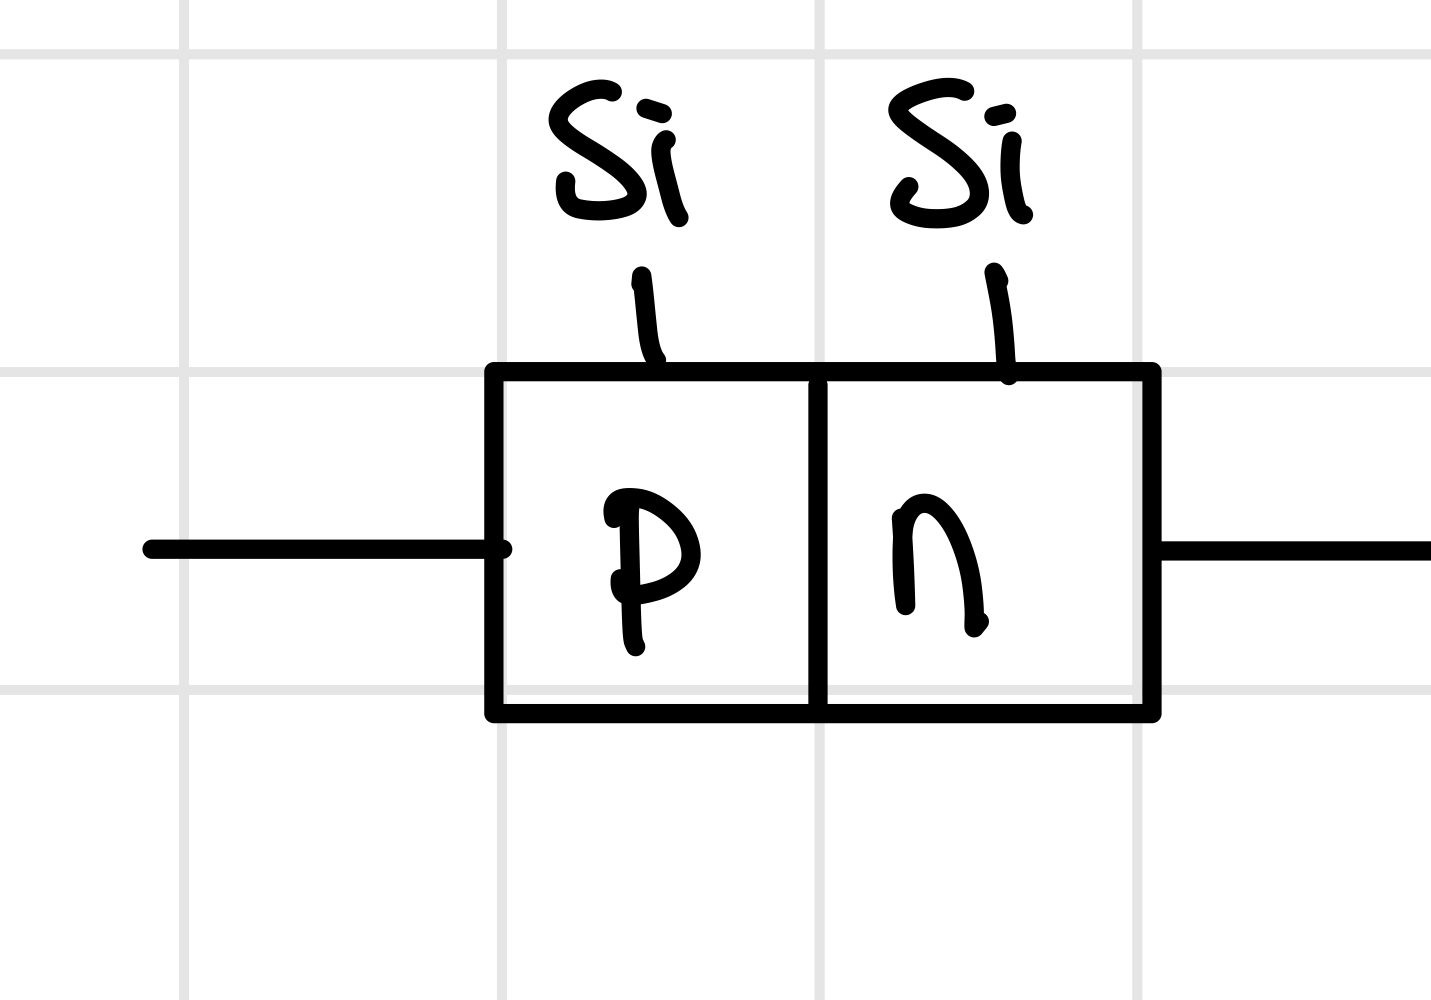
\includegraphics[scale=0.2]{Bilder/SamtaleTema6/diode.jpeg}
    \caption{diode av typen p-n}
    \label{fig:p-n}
\end{figure}

Dioden består av halvleder materiale, som vi har dopet med noen urenheter. Dopingen gjør i prinsipp at vi hever ferminivået $E_F$. I p-delen ligger $E_F$ nærmest valensbåndet, og i n-delen ligger $E_F$ nærmest ledningsbåndet.

Forenklede bånddiagram plotter bare valence band max (\textbf{VBM} - toppen av valensbåndet) og conduction band min (\textbf{CBM} bunnen av ledningsbånde). Dette blir sende ut som i figur \ref{fig:forenkl}.

\begin{figure}[!htb]
    \centering
    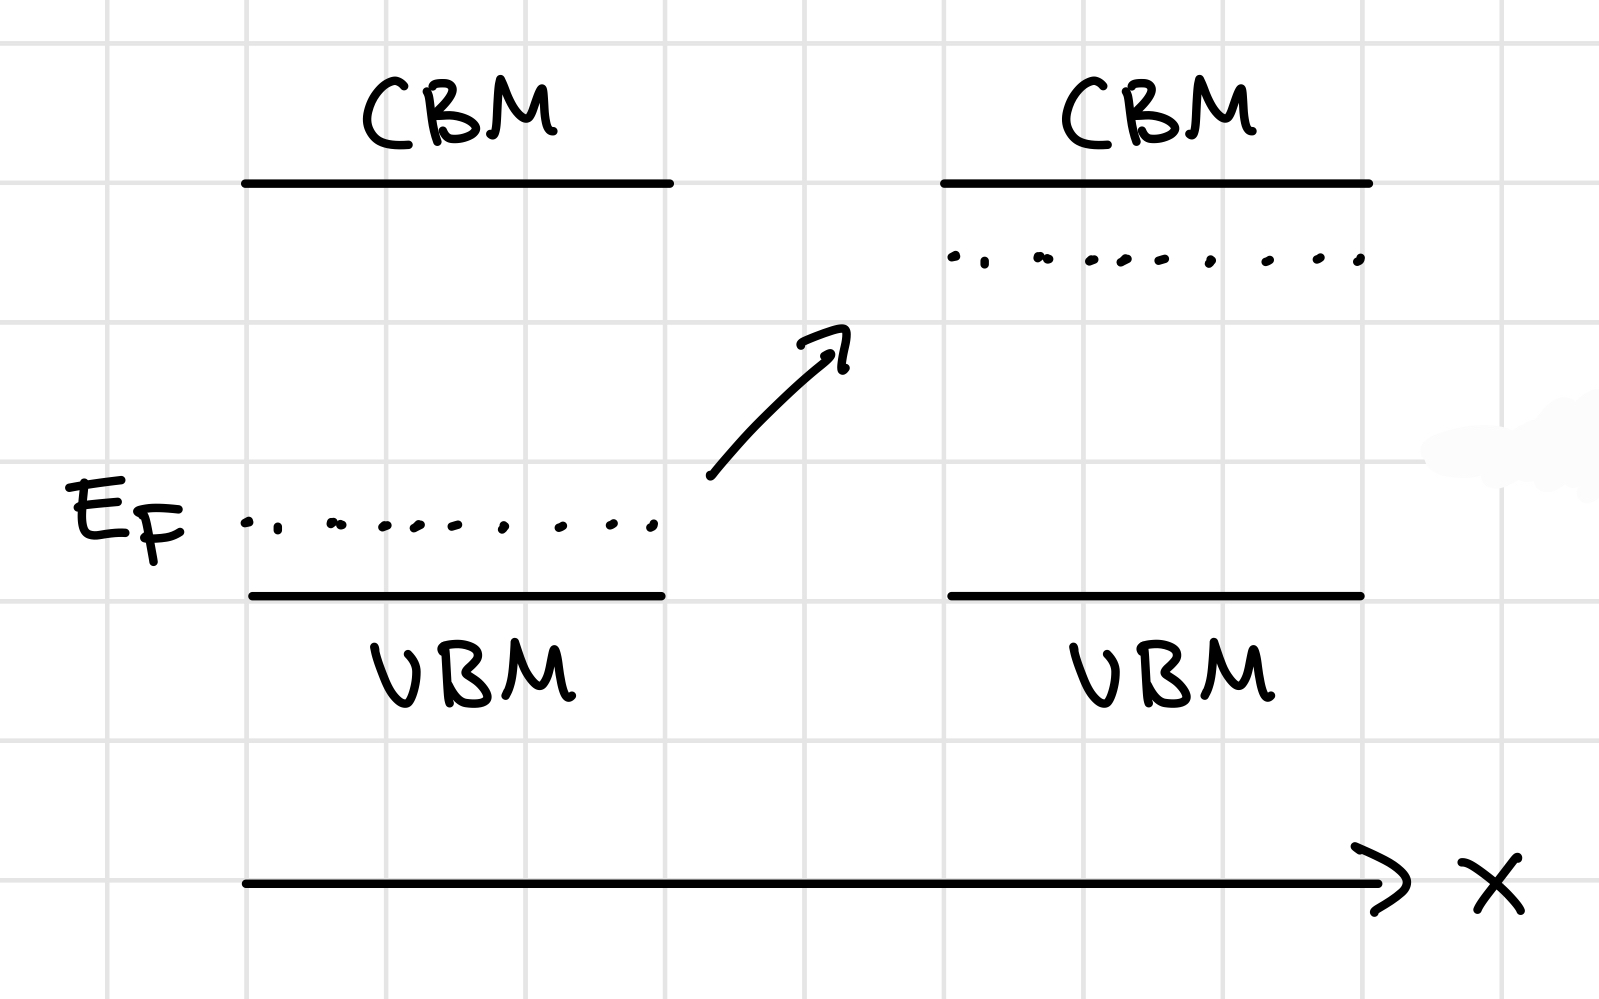
\includegraphics[scale=0.2]{Bilder/SamtaleTema6/forenklet.jpeg}
    \caption{Forenklet bånd diagram}
    \label{fig:forenkl}
\end{figure}

Disse blir ofte slått sammen og $E_F$ blir sentrert for de to delene. Illustrasjonen i figur \ref{fig:forenkl-sammen} viser hvordan dette ser ut.

\begin{figure}[!htb]
    \centering
    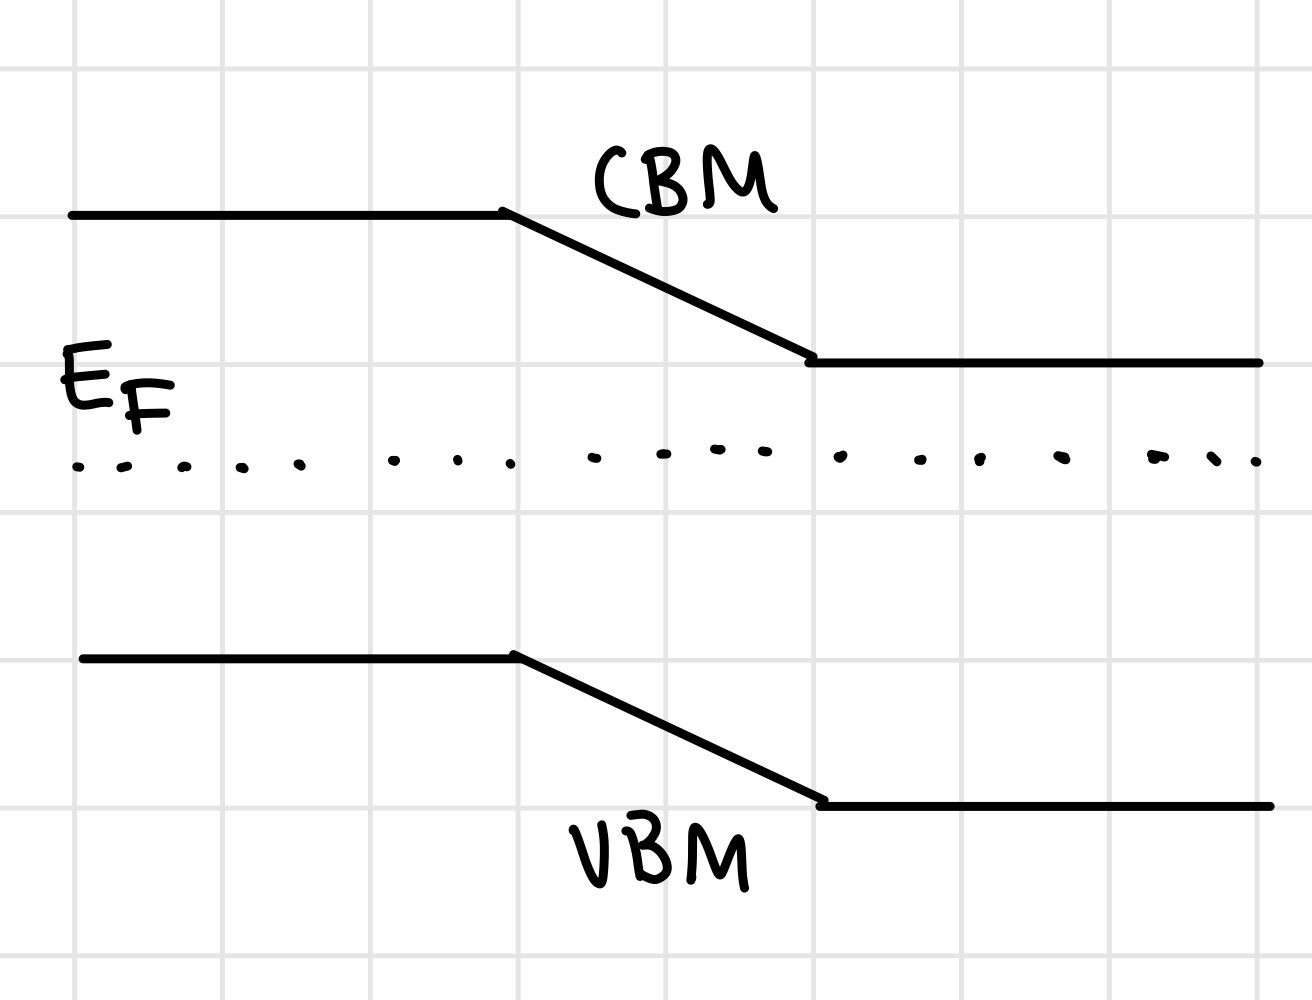
\includegraphics[scale=0.2]{Bilder/SamtaleTema6/forenklet-sentrert.jpeg}
    \caption{Forenklet bånddiagram med sentrert $E_F$}
    \label{fig:forenkl-sammen}
\end{figure}